\documentclass[12pt,a4paper]{report}

%adjust your page margins here
\usepackage[top=0.60in, bottom=0.70in, left=0.8in,right=0.80in]{geometry} % setting the page alignment with this package
\usepackage[pdftex]{graphicx} %for embedding images
\usepackage[explicit]{titlesec}
\usepackage{tocloft}

\titleformat{\chapter}[display]{\bfseries\centering}{\begin{flushright}{\huge Chapter \thechapter} \end{flushright}}{1em}{\Huge #1}


%\titleformat{\chapter}[display]
%{\normalfont\huge\bfseries\centering}{\chaptertitlename\ \thechapter}{20pt}{\Huge}

\usepackage[%dvips, % commented for pdflatex
bookmarks,  colorlinks=false]{hyperref} %for creating links in the pdf version and other additional pdf attributes, no effect on the printed document
\hypersetup{%
    pdfborder = {0 0 0}
}
\usepackage[final]{pdfpages} %for embedding another pdf, remove if not required
\usepackage{float} %used for figure placement with H as a parameter
\usepackage{hyperref}
\usepackage{pslatex} % for times new roman, old package, but works
\usepackage{array} % for making text bold in table
\usepackage{setspace}
\usepackage{float}
\usepackage{enumerate}
\usepackage{longtable}

\usepackage[font=small,labelfont=bf]{caption}
\def\figurename{\textbf{Figure }}

\usepackage{listings}
\usepackage{color}

\definecolor{dkgreen}{rgb}{0,0.6,0}
\definecolor{gray}{rgb}{0.5,0.5,0.5}
\definecolor{mauve}{rgb}{0.58,0,0.82}
 
\lstset{ %
  language=Java,                % the language of the code
  basicstyle=\footnotesize,           % the size of the fonts that are used for the code
  numbers=left,                   % where to put the line-numbers
  numberstyle=\tiny\color{gray},  % the style that is used for the line-numbers
  stepnumber=1,                   % each line is numbered
  numbersep=5pt,                  % how far the line-numbers are from the code
  backgroundcolor=\color{white},      % choose the background color. You must add \usepackage{color}
  showspaces=false,               % show spaces adding particular underscores
  showstringspaces=false,         % underline spaces within strings
  showtabs=false,                 % show tabs within strings adding particular underscores
  frame=single,                   % adds a frame around the code
  rulecolor=\color{black},        % if not set, the frame-color may be changed on line-breaks within not-black text (e.g. commens (green here))
  tabsize=2,                      % sets default tabsize to 2 spaces
  captionpos=b,                   % sets the caption-position to bottom
  breaklines=true,                % sets automatic line breaking
  breakatwhitespace=false,        % sets if automatic breaks should only happen at whitespace
  title=\lstname,                   % show the filename of files included with \lstinputlisting;
                                  % also try caption instead of title
  keywordstyle=\color{blue},          % keyword style
  commentstyle=\color{dkgreen},       % comment style
  stringstyle=\color{mauve},         % string literal style
  escapeinside={\%*}{*)},            % if you want to add a comment within your code
  morekeywords={*,...}               % if you want to add more keywords to the set
}
%For the header and footer
\usepackage{fancyhdr}
\fancypagestyle{plain}{
\fancyfoot[L]{\emph{Designed By: Vivek Shekhawat (21ESKIT122)}} % except the center
\fancyfoot[R]{\thepage}
\renewcommand{\headrulewidth}{0.4pt}
\renewcommand{\footrulewidth}{0.4pt}
}
\pagestyle{fancy}
\rhead{\emph{}}
\setlength\headheight{14.5pt}
\fancyfoot[LO,LE]{\emph{Designed By: Vivek Shekhawat (21ESKIT122)}}
\cfoot{}
\fancyfoot[R]{\thepage}
\renewcommand{\headrulewidth}{0.4pt}
\renewcommand{\footrulewidth}{0.4pt}
%For the header and footer Over

%Page Border
\usepackage{pgf}
\usepackage{pgfpages}

\pgfpagesdeclarelayout{boxed}
{
  \edef\pgfpageoptionborder{0pt}
}
{
  \pgfpagesphysicalpageoptions
  {%
    logical pages=1,%
  }
  \pgfpageslogicalpageoptions{1}
  {
    border code=\pgfsetlinewidth{2pt}\pgfstroke,%
    border shrink=\pgfpageoptionborder,%
    resized width=.95\pgfphysicalwidth,%
    resized height=.95\pgfphysicalheight,%
    center=\pgfpoint{.5\pgfphysicalwidth}{.5\pgfphysicalheight}%
  }%
}
\pgfpagesuselayout{boxed}
\setlength{\parindent}{1cm}
%GLOBAL SETTINGS OVER, DOCUMENT BEGINS

\begin{document}
\renewcommand\bibname{References}
\lhead{ }

\newpage
\begin{center}
\thispagestyle{empty}
\Large{\textbf{ \emph{A PROJECT REPORT}}\\[0.3cm]}
\Large{\textbf{ \emph{on}}\\[0.3cm]}
\LARGE{\textsc {\textbf{``QUIZ APP - INTERACTIVE QUIZ PLATFORM''}}}\\[0.3cm]

\vspace{.30cm}
\emph{Submitted in Partial fulfillment for the award of degree of}\\
\vspace{.30cm}
\textbf{\emph{Bachelor of Technology}}\\
\textbf{\emph{(INFORMATION TECHNOLOGY)}}\\[0.3cm]

\vspace{1cm}

\centering

\includegraphics[scale=0.8]{project/images/download}\\

\vspace{1cm}

\Large{\textbf{Mentor:\hspace{11cm}Submitted By:}}\\
\Large{Ms. Anjali Pandey\hspace{8cm}Vivek Shekhawat}\\
\Large{Assistant Professor-II\hspace{8.4cm}21ESKIT122}\\
\raggedright
\Large{SKIT, Jaipur}\\
\vspace{3cm}

\centering

\Large{\textbf{Department of Information Technology}}\\
\vspace{0.3cm}
\Large{\textbf{Swami Keshvanand Institute of Technology, Management \& Gramothan, Jaipur }}\\
\vspace{0.3cm}
\Large{\textbf{Ramnagaria (Jagatpura), Jaipur-302017}}
\vspace{0.3cm}
\large{\textbf{\\December, 2023}}\\
\vspace{3cm}


\end{center}

\pagenumbering{roman} 

\begin{center}

\vspace{7cm}
\LARGE{\textbf{ACKNOWLEDGEMENT}}\\[1cm]
\end{center}
\linespread{1}

\large{\paragraph{}
I extend my sincere gratitude to all those who have played crucial roles in the successful development of the Quiz App project for the Bachelor of Technology (B.Tech.) program. This achievement would not have been possible without the unwavering support, encouragement, and expertise of various individuals and organizations.}

\large{\paragraph{}
A special acknowledgment is extended to \textbf{SKIT College} for providing the essential platform and resources that facilitated the practical application of theoretical knowledge in the development of the Quiz App. I am sincerely grateful for the guidance and mentorship of \textbf{Mr. Subham Gupta Sir}, whose insights have been invaluable throughout the development process. Their expertise has significantly enriched my understanding of the subject matter.}

\large{\paragraph{}
I express my deep appreciation to the esteemed faculty at \textbf{Swami Keshvanand Institute of Technology Management \& Gramothan}, particularly \textbf{Dr. (Prof.) Anil Chaudhary}, Head of the Department of Information Technology, for their continuous guidance and mentorship. Dr. Chaudhary's leadership has played a pivotal role in creating an environment conducive to academic and project excellence. Special thanks to \textbf{Ms. Anjali Pandey} for her continuous support as well, contributing to the dynamic learning atmosphere.}

\large{\paragraph{}
I would also like to express my appreciation to my peers and colleagues who actively participated in discussions, shared innovative ideas, and collaborated on various aspects of the project development. The collective effort and camaraderie among us have contributed to a holistic learning and development experience.}

\large{\paragraph{}
Lastly, I extend my sincere thanks to my family and friends for their steadfast encouragement and understanding during the demanding phases of this B.Tech project. Their unwavering support has been a constant source of motivation.}

\large{\paragraph{}
In conclusion, I acknowledge the collective efforts of all those who have played a role, directly or indirectly, in the successful completion of this project. Your contributions are deeply appreciated and have been instrumental in shaping this development journey.}

\begin{flushright}
{
\vspace{1cm}
\textbf{VIVEK SHEKHAWAT}\\
\textbf{21ESKIT122}\\
\vspace{.5cm}
}
\end{flushright}
\newpage


\cleardoublepage
\tableofcontents

\clearpage 
\pagenumbering{arabic}  % Move this line to here

\chapter{CERTIFICATE}

\begin{figure}[h]
    \centering
    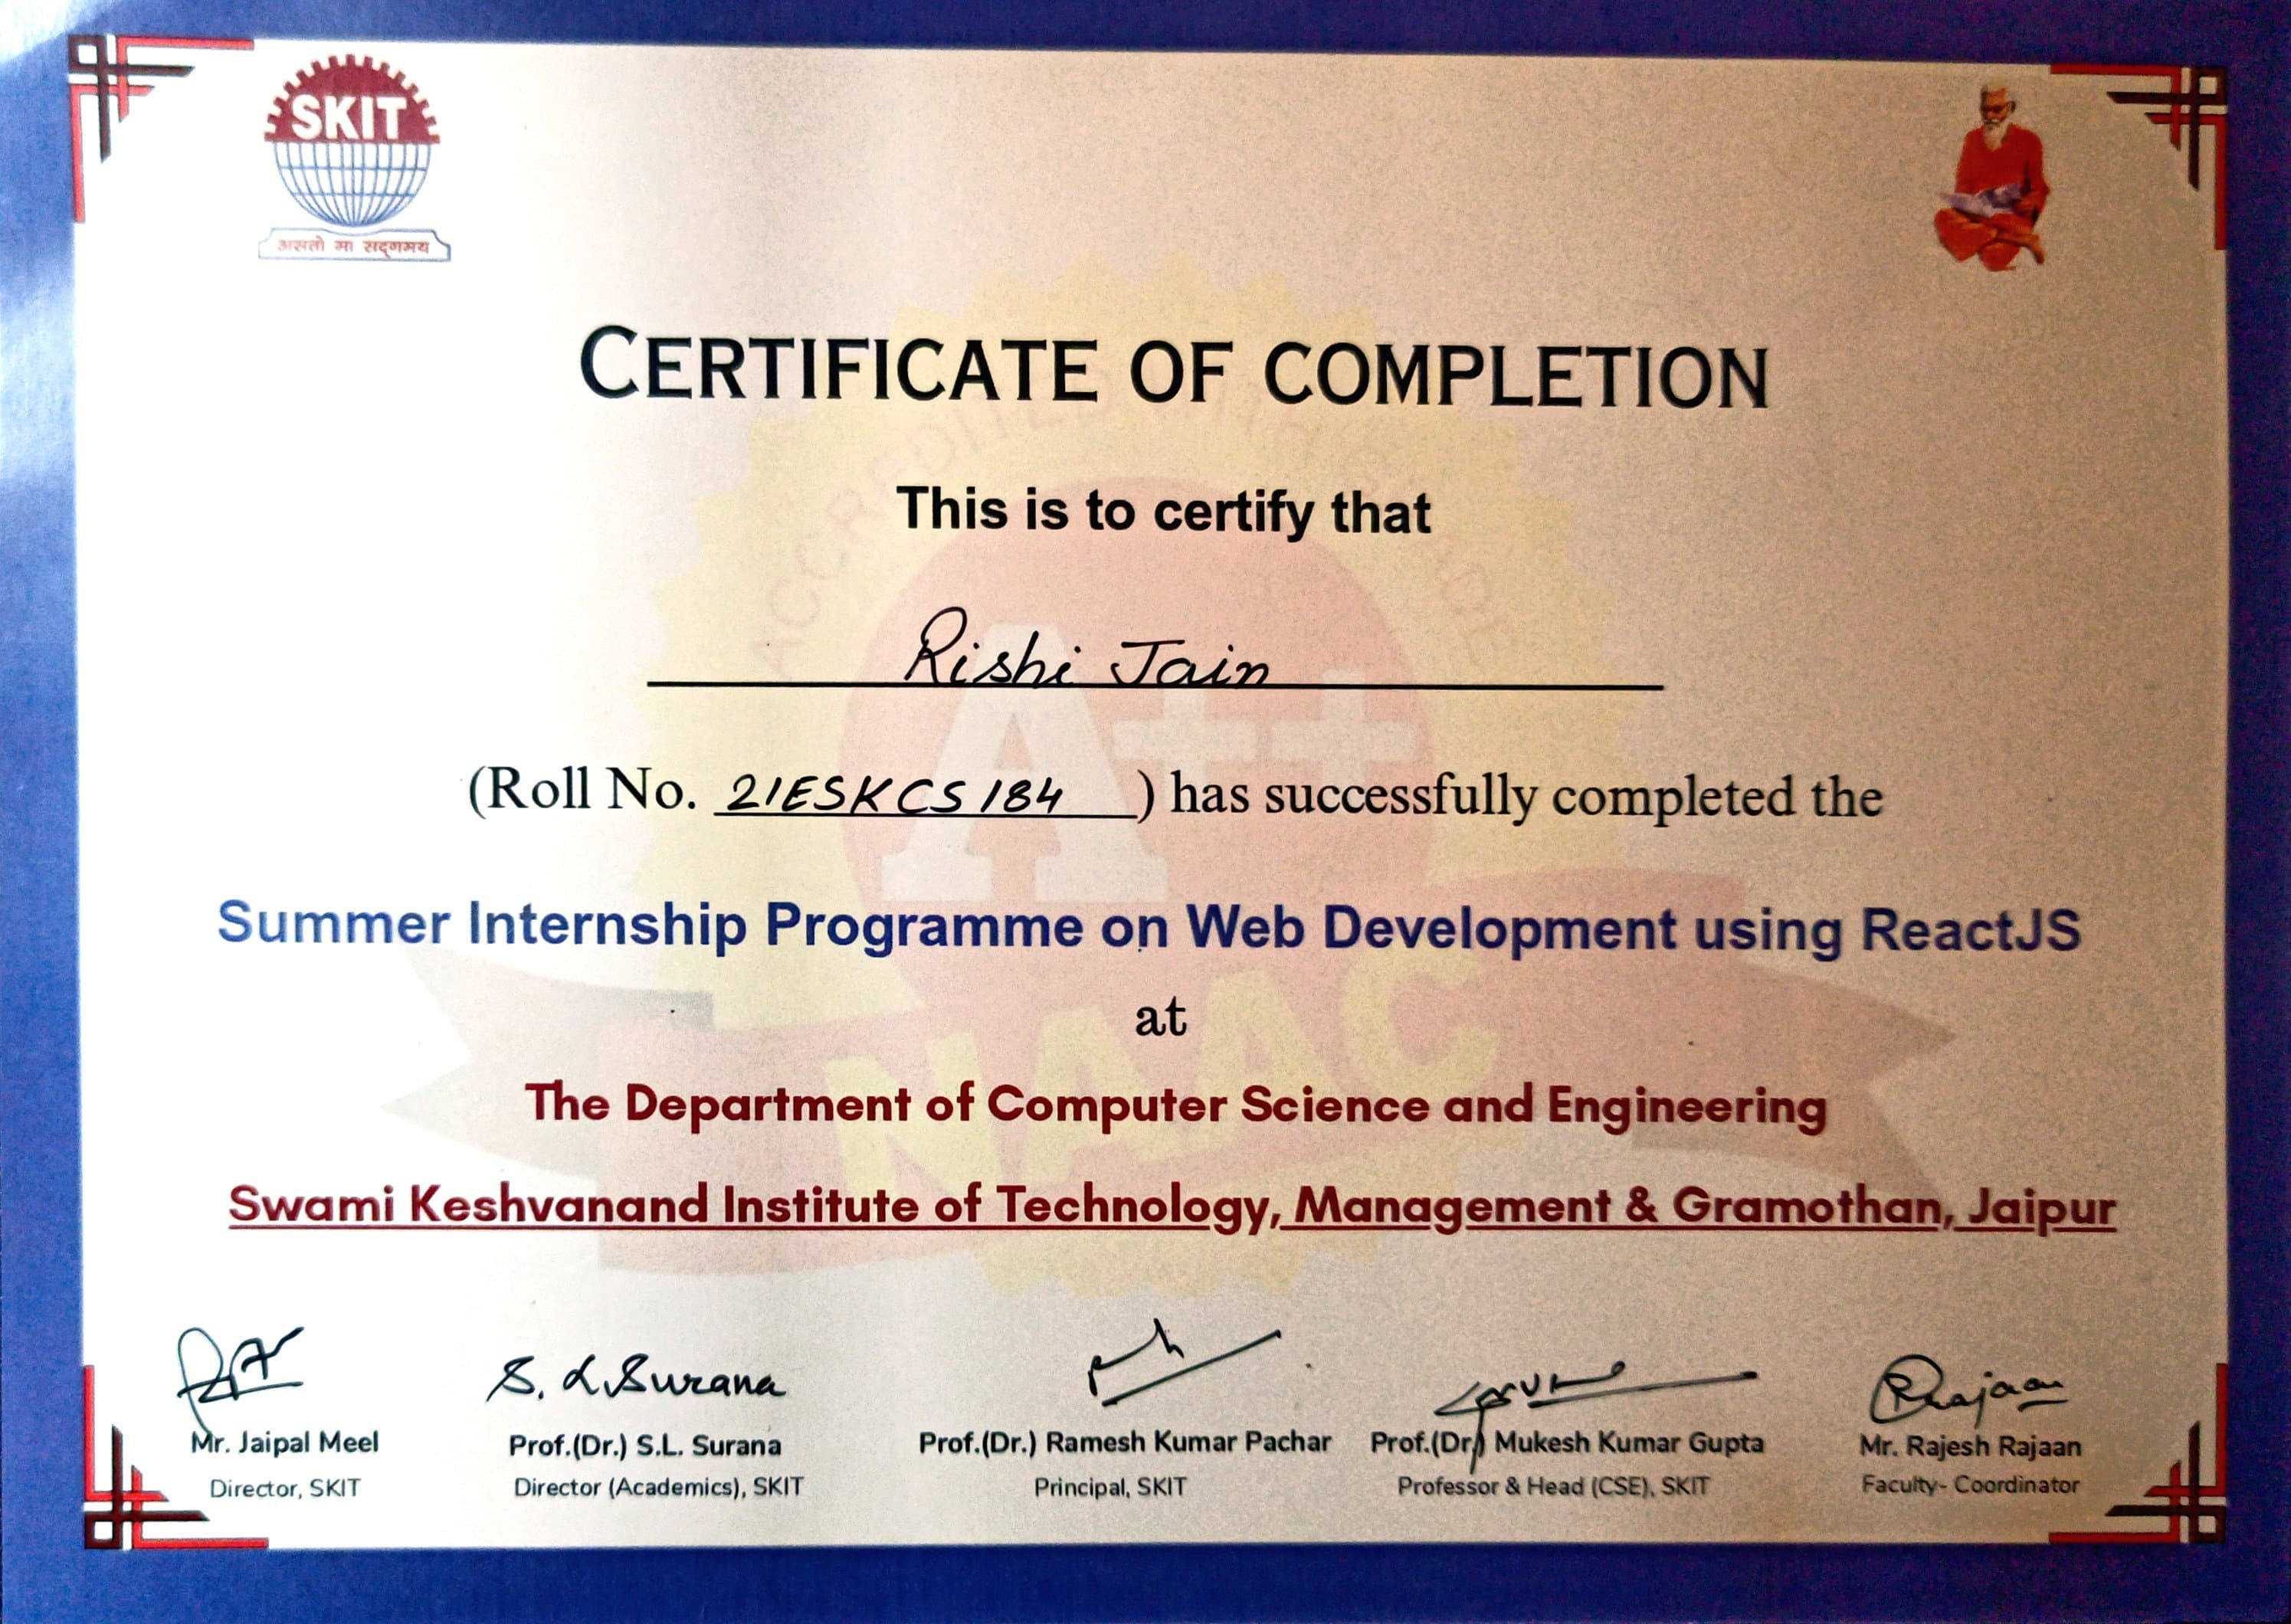
\includegraphics[scale=0.13]{project/images/front.jpg}
    \caption{Front Side of the Certificate}
\end{figure}

\begin{figure}[h]
    \centering
    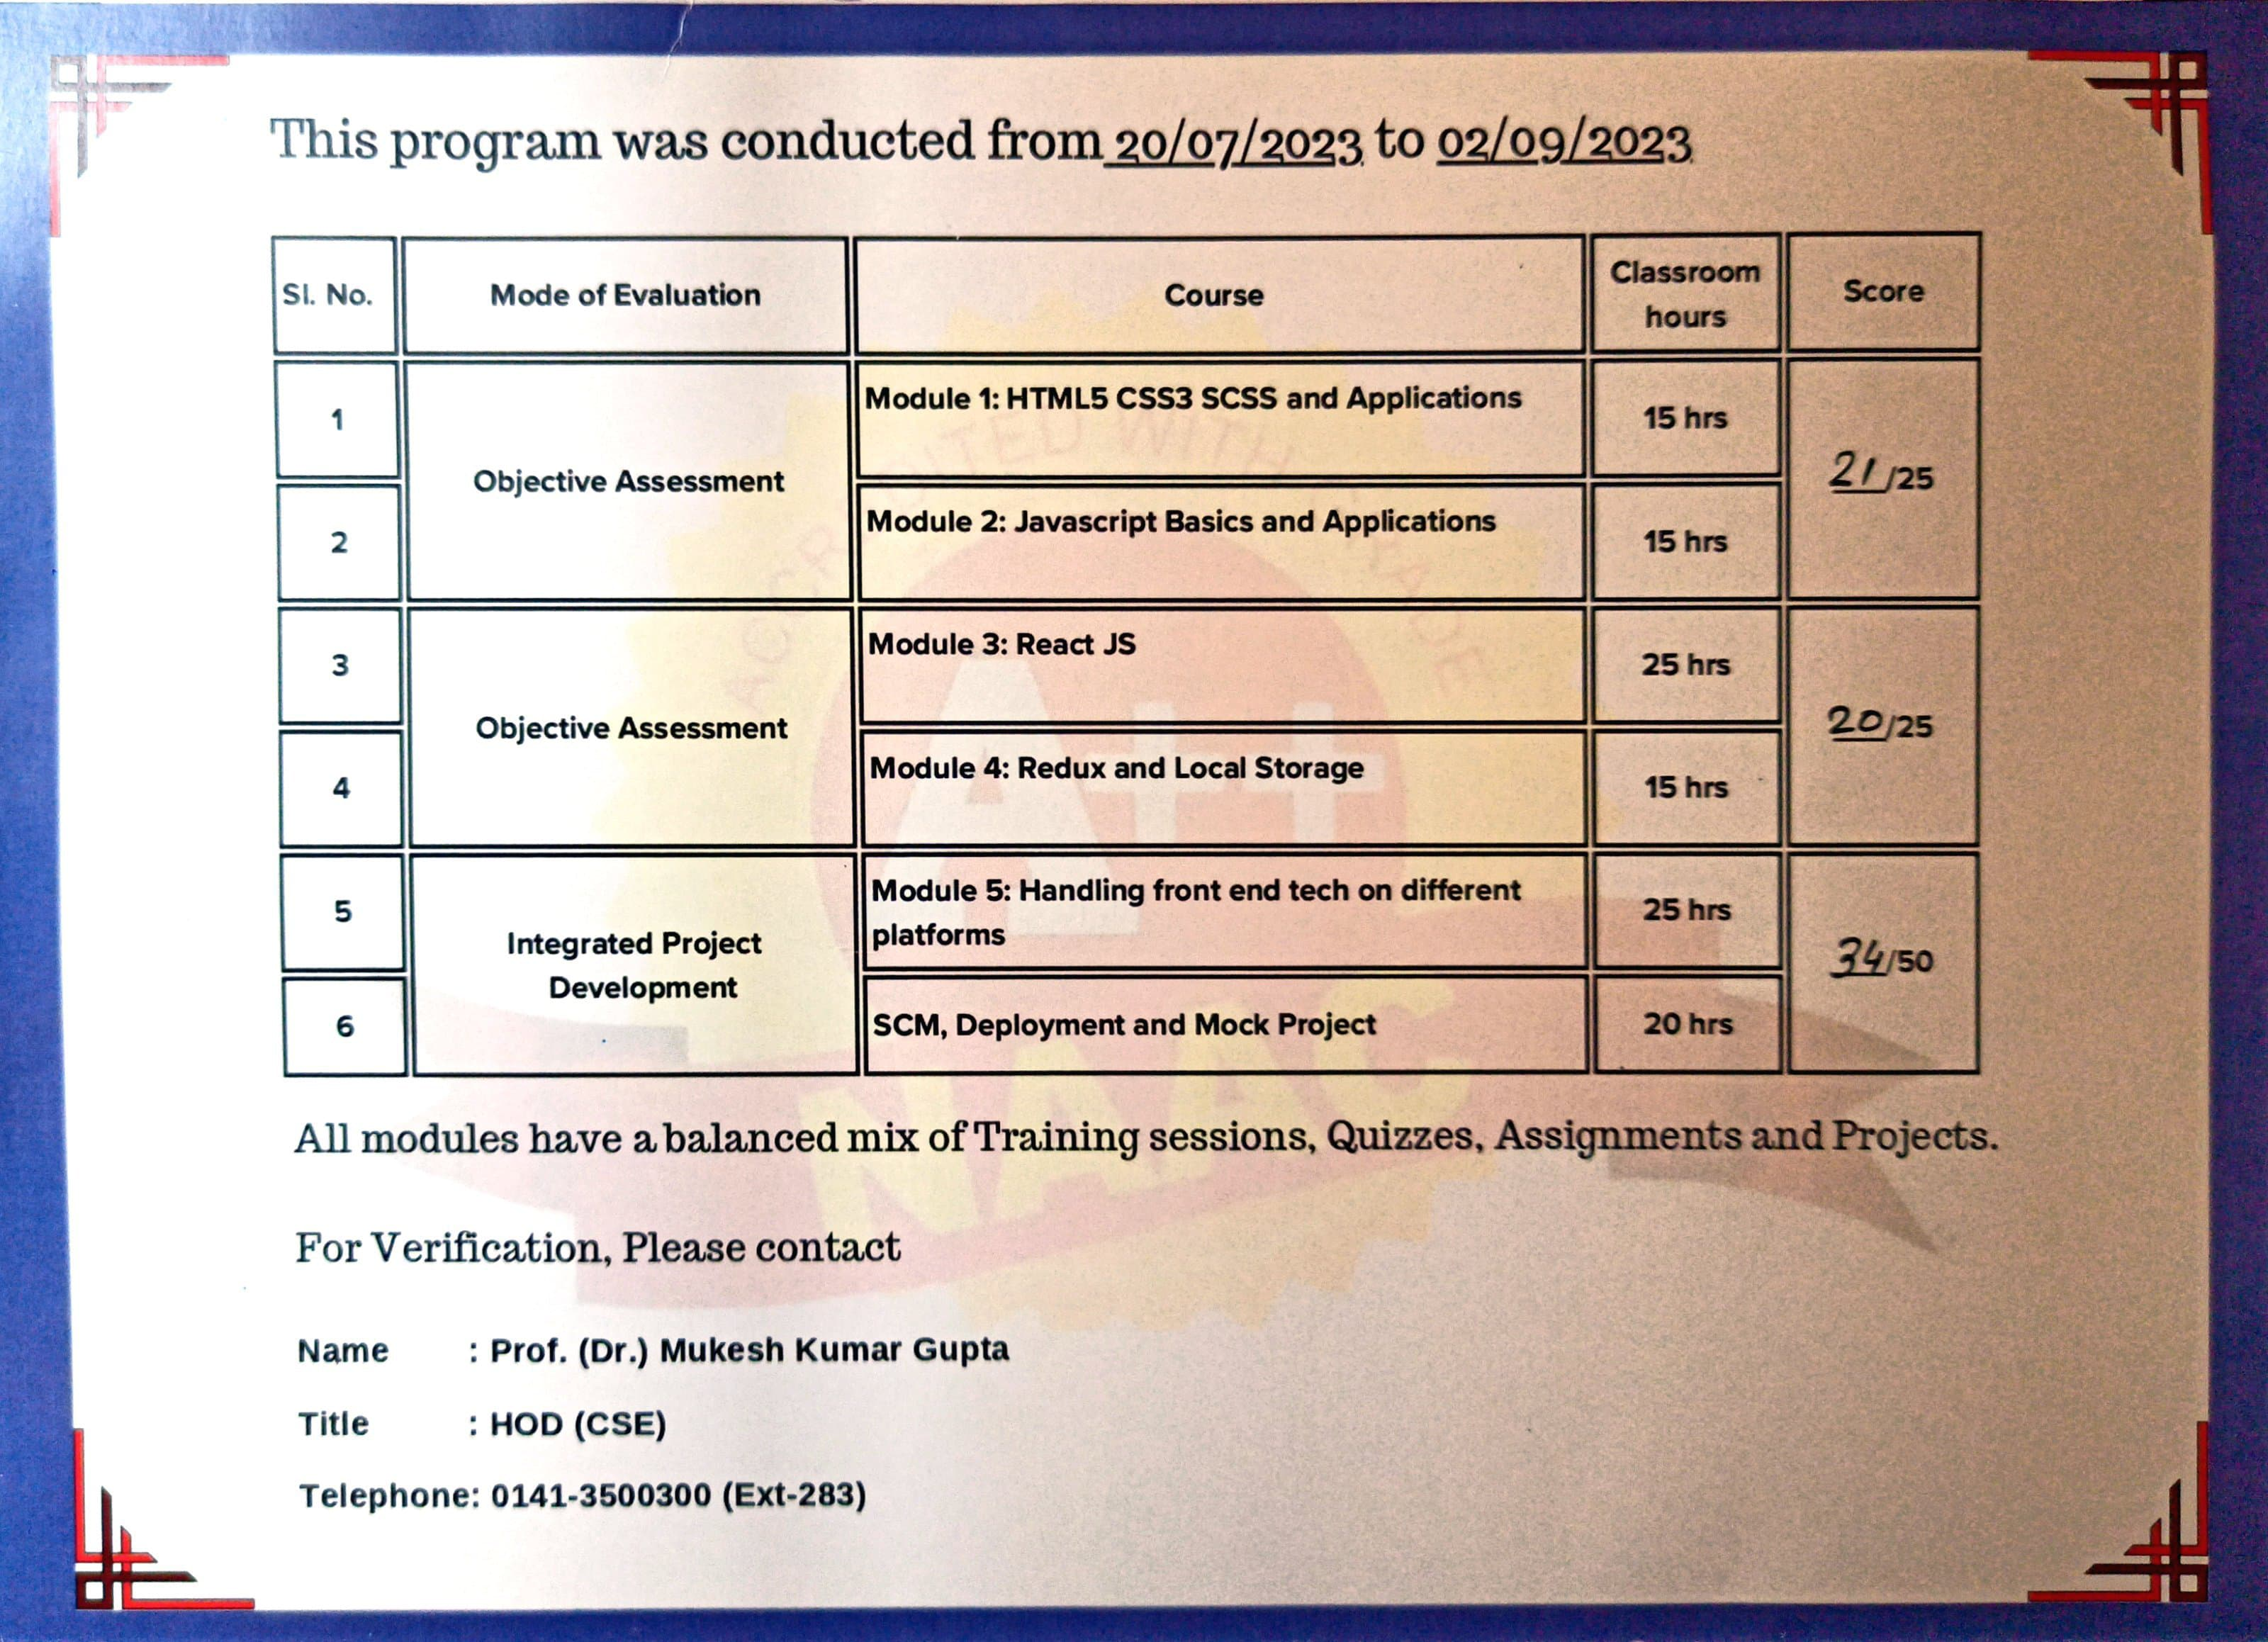
\includegraphics[scale=0.13]{project/images/PICHE.jpg}
    \caption{Back Side of the Certificate}
\end{figure}

\chapter{INTRODUCTION}

\large{\paragraph{}
The Quiz App is a dynamic educational platform crafted using modern web technologies, primarily JavaScript, HTML, and CSS. Leveraging the power of React for the frontend and Axios for API integration, this application stands at the forefront of interactive and user-centric learning experiences. The integration of three key APIs—one for student data, another for teacher functionalities, and the third for accurate answers and marks calculation—positions the Quiz App as a comprehensive and efficient tool for both students and faculty.}

\large{\paragraph{}
In the ever-evolving landscape of education technology, the Quiz App redefines the quiz-taking process. Designed with a focus on user experience, the application allows students to seamlessly choose quizzes from various subjects, answer questions, and submit responses. Simultaneously, faculty members can manage quiz content, add new subjects, and ensure accurate evaluation through real-time data synchronization.}

\large{\paragraph{}
Built on JavaScript, HTML, and CSS, the Quiz App is a testament to the versatility of these technologies. React, a JavaScript library, empowers the frontend with its component-based architecture, providing a responsive and dynamic user interface. The integration of Axios facilitates the seamless communication between the application and three distinct APIs, each serving a crucial role in enhancing the overall functionality of the Quiz App.}

\section{Intended Users}
The Quiz App caters to the following primary user categories:

\begin{enumerate}
    \item \textbf{Student Users:} Students engage with the application to register, log in, and participate in quizzes. The student API enables them to access quiz information, submit responses, and receive feedback.

    \item \textbf{Teacher Users:} Faculty members utilize the teacher API to manage quiz content. This includes adding new subjects, creating questions, and organizing quizzes. The application's design ensures a user-friendly interface for efficient content management.

\end{enumerate}

\section{Tools and Technologies Used}
The Quiz App harnesses the following tools and technologies for its development:

\begin{itemize}
    \item \textbf{React:} The frontend is developed using React, a JavaScript library known for building dynamic user interfaces.

    \item \textbf{Axios:} This technology facilitates API integration, allowing smooth communication between the application and three distinct APIs—student, teacher, and answers/marks.

    \item \textbf{JavaScript, HTML, CSS:} These foundational web technologies form the backbone of the Quiz App, providing the necessary structure, styling, and interactivity.

\end{itemize}

\section{Key Features}
The Quiz App boasts several key features to enhance the learning and quiz-taking experience:

\begin{enumerate}
    \item \textbf{User-Friendly Interface:} The application is designed with a focus on user experience, ensuring an intuitive and navigable interface for both students and faculty members.

    \item \textbf{Quiz Selection and Submission:} Students can choose quizzes, answer questions, and submit responses for evaluation. The integration with the student API enables seamless access to quiz data.

    \item \textbf{Quiz Management:} Faculty members utilize the teacher API to manage quiz content, adding new subjects, creating questions, and organizing quizzes. This feature ensures an efficient workflow for educators.

    \item \textbf{Real-Time Data Synchronization:} The application's integration with three APIs ensures real-time updates and synchronization, providing accurate information for students and facilitating efficient content management for teachers.

\end{enumerate}

\section{Future Aspects}
As the Quiz App evolves, potential future enhancements may include:

\begin{enumerate}
    \item \textbf{Certificate Options:} Integration of a certificate generation system based on student performance, adding a recognition element to successful quiz completion.

    \item \textbf{Multiple User Collaboration:} Expanding the application to support collaborative quiz-taking experiences, enabling multiple users to participate in quizzes simultaneously.

    \item \textbf{Extended Functionality:} Continued integration with additional APIs or technologies to enhance the educational offerings of the Quiz App.

\end{enumerate}

\section{Uniqueness}
The Quiz App stands out in the following ways:

\large{\paragraph{}}

\textbf{API Integration:} The application's utilization of three distinct APIs—student, teacher, and answers/marks—sets it apart, ensuring a comprehensive and integrated educational platform.

\large{\paragraph{}}

\textbf{JavaScript and React Foundation:} Built on JavaScript and leveraging the power of React, the Quiz App showcases the strength of these technologies in creating dynamic and responsive web applications.

\large{\paragraph{}}

\textbf{User-Centric Design:} With a focus on user experience, the Quiz App prioritizes a user-friendly interface, making quiz-taking and content management intuitive and enjoyable for both students and faculty.

\large{\paragraph{}}

In conclusion, the Quiz App's adoption of JavaScript, HTML, CSS, React, and Axios, coupled with its API integration and user-centric design, positions it as a cutting-edge educational tool. As the application continues to evolve, it remains committed to providing a seamless and interactive learning experience for students and faculty members alike.

\chapter{METHODOLOGY}
\section{Software Model Used}
\textbf{Agile Methodology}\\
Agile methodology is the chosen approach for the development of the Quiz App, embracing the principles of flexibility, iterative development, and responsiveness to changing requirements. Unlike the traditional Waterfall model, Agile promotes continuous collaboration between cross-functional teams, allowing for incremental development and continuous user feedback. This iterative approach aligns well with the dynamic nature of educational technology projects.

\begin{figure}[h!]
    \centering
    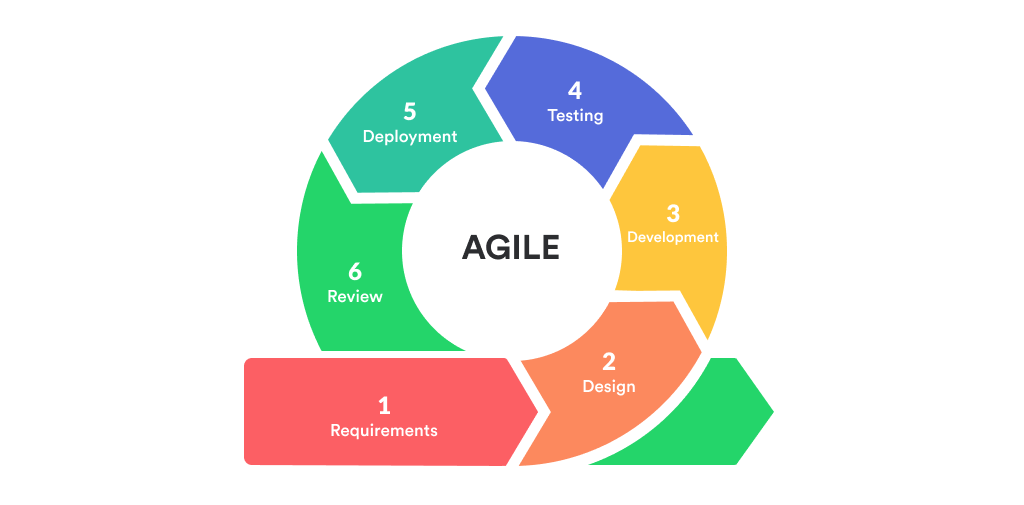
\includegraphics[scale=0.5]{project/images/Agile1.png}
    \caption{AGILE METHODOLOGY}
\end{figure}

The Agile methodology facilitates the seamless integration of different components and features, ensuring a cohesive and adaptable development process.

\section{Product User Interfaces}
The Quiz App's user interfaces are designed to provide an engaging and intuitive experience for both students and faculty members. Let's explore the various interfaces:

\subsection{Welcome Page}
\begin{center}
    \includegraphics[scale=0.4]{project/images/WELCOME.png}
\end{center}

The welcome page serves as the entry point for users, providing a visually appealing and informative introduction to the Quiz App. It sets the tone for a positive user experience.

\subsection{Login Page}
\begin{center}
    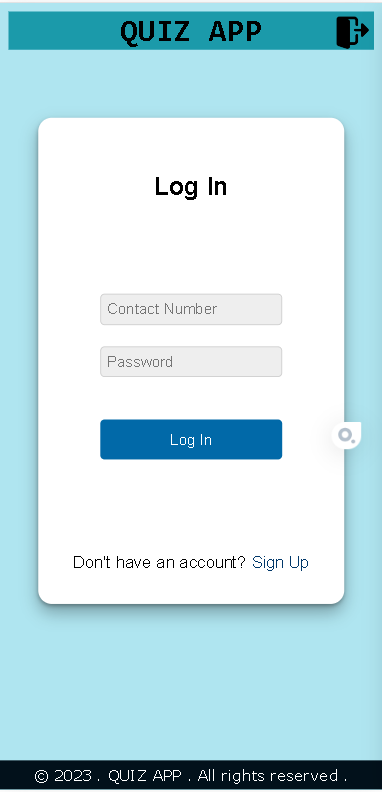
\includegraphics[scale=0.4]{project/images/LOGIN.png}
\end{center}

The login page allows users to securely access their accounts. Students and faculty members can enter their credentials to log in and access personalized features based on their roles.

\subsection{Register Page}
\begin{center}
    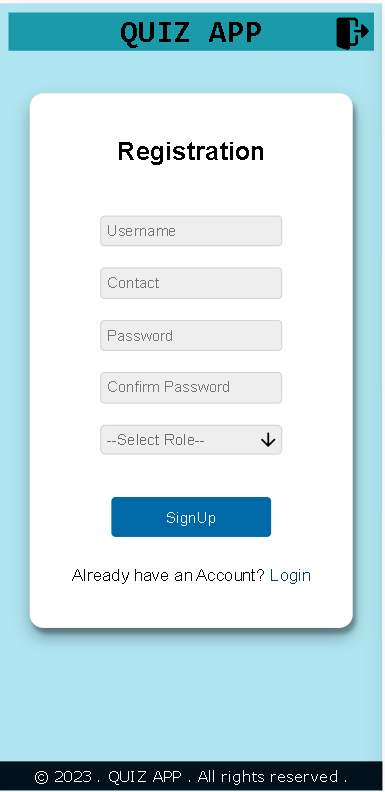
\includegraphics[scale=0.4]{project/images/REGISTER.png}
\end{center}

For new users, the register page offers a straightforward registration process. Students and faculty can create accounts by providing essential details, ensuring a seamless onboarding experience.

\subsection{Student Interface - Subject Selection}
\begin{center}
    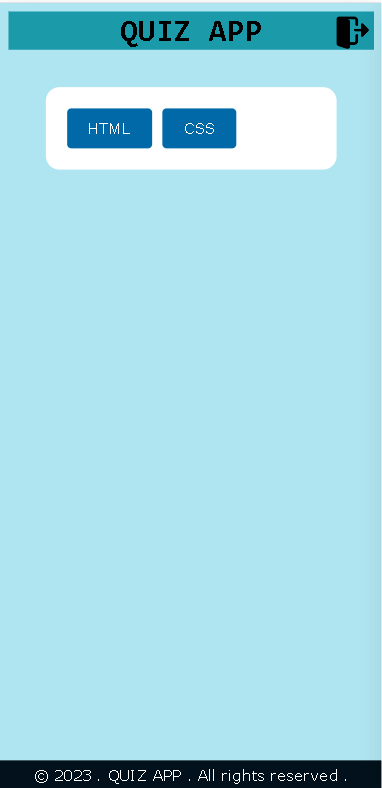
\includegraphics[scale=0.4]{project/images/QUIZ PANEL.png}
\end{center}

Students can choose quizzes based on subjects of their interest. The interface provides a user-friendly way to navigate through available subjects and select quizzes to participate in.

\subsection{Student Interface - Specific Subject Questions}
\begin{center}
    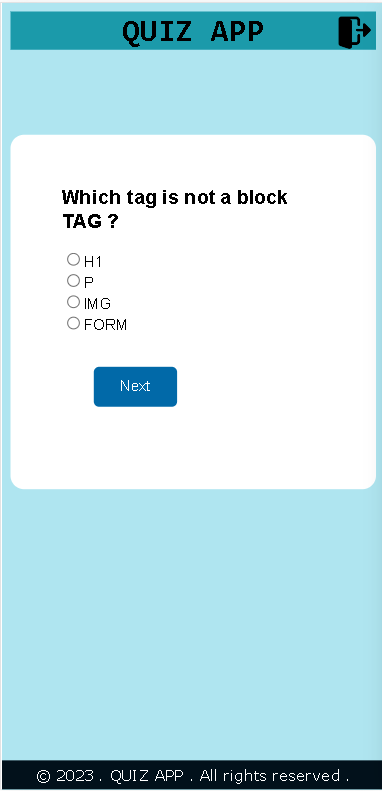
\includegraphics[scale=0.4]{project/images/QUIZ PANEL2.png}
\end{center}

For a more targeted quiz experience, students can opt for specific subject questions. This interface displays questions related to a particular subject, allowing students to focus on their areas of study.

\subsection{Faculty Interface - Add Subject}
\begin{center}
    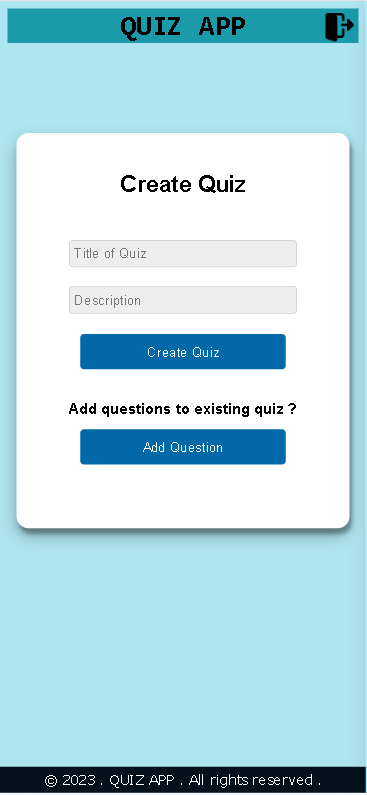
\includegraphics[scale=0.4]{project/images/ADD SUBJECT.png}
\end{center}

Faculty members have the capability to enrich the Quiz App by adding new subjects. This interface streamlines the process, ensuring efficient management of the available subjects.

\subsection{Faculty Interface - Add Question}
\begin{center}
    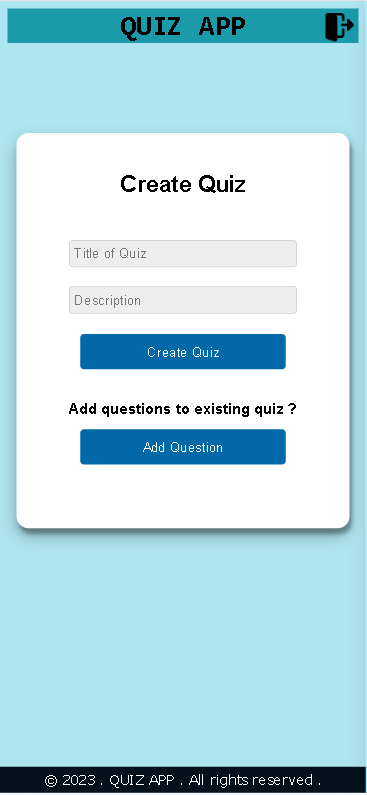
\includegraphics[scale=0.4]{project/images/ADD SUBJECT.png}
\end{center}

Facilitating continuous improvement, faculty members can contribute to the question database by adding new questions. This interface provides a structured form for adding questions, ensuring consistency in data entry.

\section{Features}

The Quiz App incorporates several features to enhance the learning and quiz-taking experience:

\begin{enumerate}
    \item \textbf{User-Friendly Interface:} The application is designed with a focus on user experience, ensuring an intuitive and navigable interface for both students and faculty members.
    \item \textbf{Quiz Selection and Submission:} Students can choose quizzes, answer questions, and submit responses for evaluation. The integration with the student API enables seamless access to quiz data.
    \item \textbf{Quiz Management:} Faculty members utilize the teacher API to manage quiz content, adding new subjects, creating questions, and organizing quizzes. This feature ensures an efficient workflow for educators.
    \item \textbf{Real-Time Data Synchronization:} The application's integration with three APIs ensures real-time updates and synchronization, providing accurate information for students and facilitating efficient content management for teachers.
\end{enumerate}

\section{Design and Implementation Constraints}

Agile principles inherently address various constraints and promote adaptability:

\begin{enumerate}
    \item \textbf{Operating System and Device Flexibility:}
    \begin{itemize}
        \item Agile development ensures that the Quiz App remains adaptable to various operating systems and devices, providing flexibility for users with different preferences.
    \end{itemize}
    
    \item \textbf{Continuous Integration and Testing:}
    \begin{itemize}
        \item Agile's continuous integration and testing practices help identify and address potential constraints early in the development process, ensuring a robust and reliable application.
    \end{itemize}
\end{enumerate}

The Agile methodology aligns with the Quiz App's goals, fostering collaboration, adaptability, and delivering a product that meets the evolving needs of students and faculty.

\chapter{DEPENDENCIES}

\section{Assumptions and Dependencies}

One assumption about the Quiz App software is that it will be used on modern web browsers and operating systems that support React applications. Users are expected to have internet access to use the application. The Quiz App relies on Axios technology for API implementation. Internet access is essential for the proper functioning of the application.

\section{Hardware Requirements}

\begin{center}
\begin{tabular}{|p{3cm}|p{3cm}|p{3cm}|p{3cm}|}
    \hline
    \multicolumn{4}{|c|}{\textbf{Client Side}} \\
    \hline
    & Processor & RAM & Disk Space \\
    \hline 
    \textbf{Web Browsers} & Any modern web browser (e.g., Chrome, Firefox, Safari) & 2GB or more & Varies \\
    \hline
\end{tabular}
\end{center}

\section{Software Requirements}

\begin{center}
\begin{tabular}{|p{5cm}|p{10cm}|}
    \hline
    \textbf{Software} & \textbf{Description} \\
    \hline 
    \textbf{React Framework} & The Quiz App is built using React, a JavaScript library for building user interfaces. Users need a web browser that supports React applications. \\
    \hline
    \textbf{Axios Technology} & The application uses Axios for API implementation, enabling the interaction with different endpoints to retrieve and submit data. \\
    \hline
\end{tabular}
\end{center}

\chapter{NON-FUNCTIONAL REQUIREMENTS}

\raggedright

\section{Security}
\large{\paragraph{}
The Quiz App prioritizes the security of user data and maintains a secure user experience. Implementation includes measures to protect user information and ensure data integrity. Securing the connection to external services, such as the APIs used for student and faculty interactions, is achieved through secure authentication methods and encryption. Regular security audits and penetration testing are conducted to identify and mitigate vulnerabilities.}

\section{Scalability}
\large{\paragraph{}
The Quiz App is designed to handle increasing user loads, data growth, and traffic demands without compromising performance or user experience. Scalability is a crucial aspect to provide a seamless and reliable experience to users as the platform expands in size and popularity. The system architecture is optimized to scale horizontally, ensuring efficient resource utilization and load distribution.}

\section{Maintainability}
\large{\paragraph{}
To enhance maintainability, the Quiz App codebase is structured into modular components, adhering to best practices for code organization and separation of concerns. Comprehensive and up-to-date documentation is provided to assist developers in understanding and maintaining the codebase. Regular code reviews are conducted to maintain code quality and share knowledge among the development team.}

\section{Localization}
\large{\paragraph{}
The Quiz App is designed to be accessible to a diverse global audience. It implements mechanisms for translating user-generated content and quiz questions into different languages. The system detects users' preferred languages and adjusts the content and user interface accordingly. Date, time, and currency values are displayed in alignment with the user's locale to provide a personalized experience.}

\section{Performance}
\large{\paragraph{}
The Quiz App is optimized for efficient performance, ensuring quick response times for user interactions. Server response times are monitored and maintained within acceptable limits. Performance testing is conducted under varying user loads to identify and address any bottlenecks or performance issues.}

\section{Reliability}
\large{\paragraph{}
The Quiz App aims for high reliability, minimizing downtime and ensuring uninterrupted access to quizzes and user data. The system is designed with fault tolerance, and regular backups are performed to safeguard against data loss. A robust error-handling mechanism is implemented to gracefully handle unexpected issues and provide a reliable user experience.}

\section{Usability}
\large{\paragraph{}
Usability is a key focus for the Quiz App, ensuring an intuitive and user-friendly interface. User feedback is regularly collected and used to improve the user experience. The application is designed to be accessible to users with diverse technical backgrounds, and user interface elements are organized logically to facilitate easy navigation.}

\section{Accessibility}
\large{\paragraph{}
The Quiz App adheres to accessibility standards, making it usable by individuals with disabilities. The application supports screen readers, keyboard navigation, and other assistive technologies. Text and multimedia content are designed to be perceivable, operable, and understandable by a wide range of users.}

\section{Availability}
\large{\paragraph{}
The Quiz App is designed to be available 24/7, ensuring continuous access for users. Regular maintenance activities, updates, and deployments are scheduled during low-traffic periods to minimize disruptions. The system includes redundancy and failover mechanisms to mitigate the impact of potential server failures.}

\chapter{IMPLEMENTATION AND TESTING}
% \section{Database}
% \centering
% \includegraphics[scale=0.4]{project/images/Screenshot 2023-10-26 201753.png}\\
% \vspace{1cm}
% \includegraphics[scale=0.4]{project/images/Screenshot 2023-10-26 203650}\\
% \newpage
\section{Code-Snippet}
\begin{enumerate}
\item API Fetch\\
\vspace{2cm}
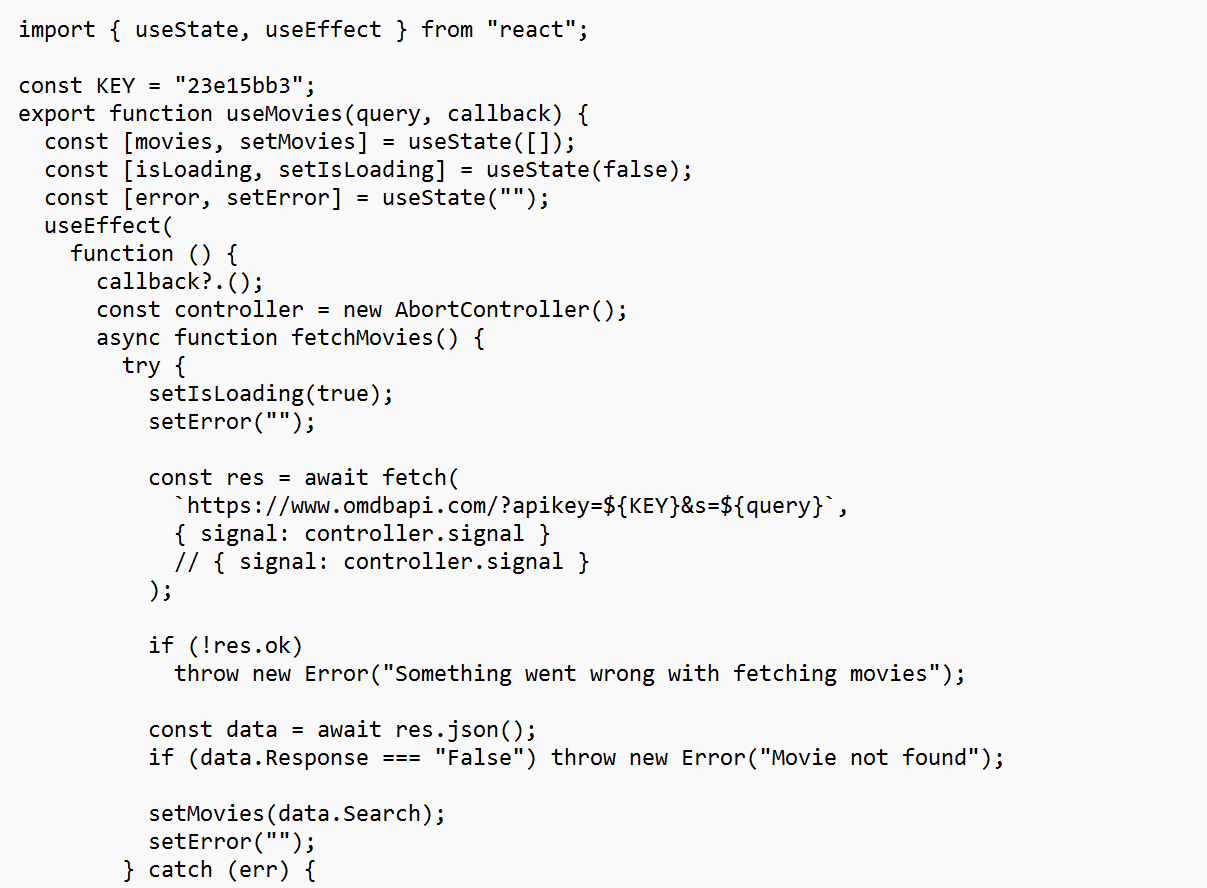
\includegraphics[height=15cm,width=17.5cm]{project/images/API.png}\\
\newpage
\item Star\\
\vspace{2cm}
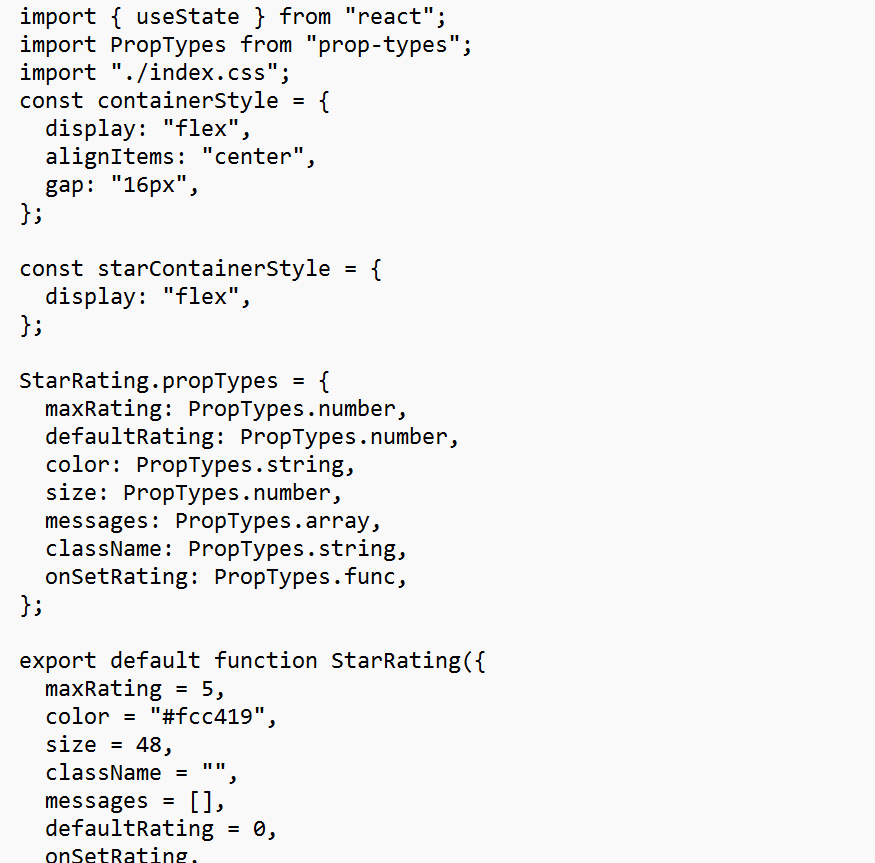
\includegraphics[height=20cm,width=16cm]{project/images/STAR.png}\\
\newpage
\item App\\
\vspace{2cm}
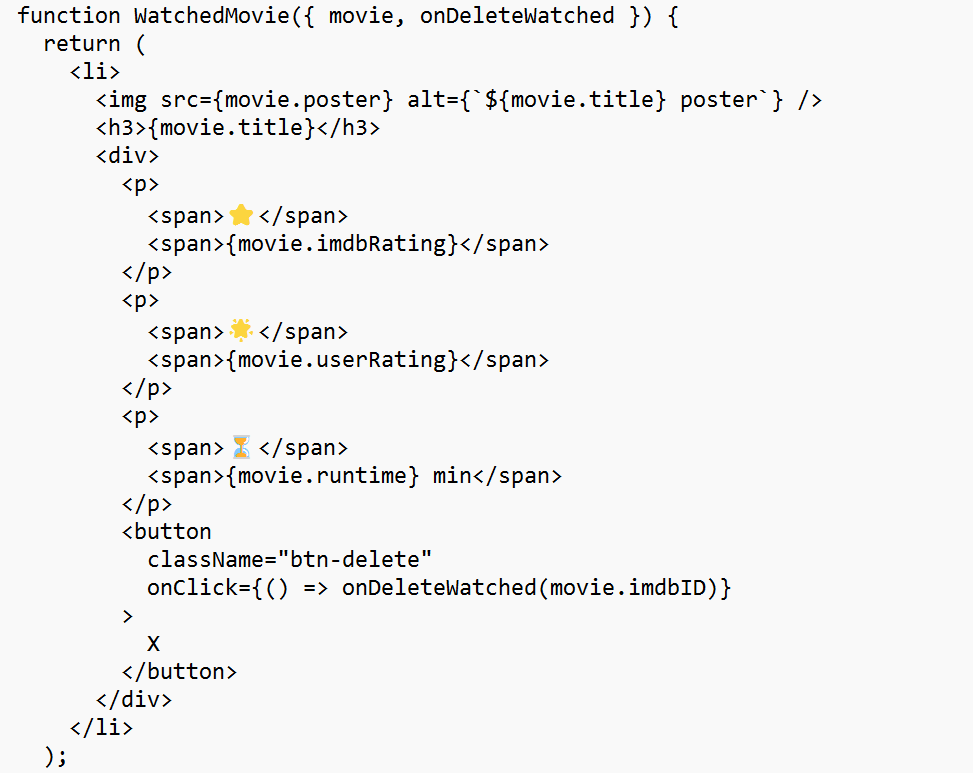
\includegraphics[height=20cm,width=16cm]{project/images/APP.png}\\
\end{enumerate}


\chapter{CONCLUSION AND FUTURE SCOPE}

\textbf{Conclusion}\\
\raggedright
\large{\paragraph{}
The "Quiz App" emerges as a successful and user-friendly solution, providing a dynamic quiz-taking experience for both students and faculty. With its intuitive interface and diverse subject options, this project simplifies the quiz process and enriches the learning experience.}
\large{\paragraph{}
In conclusion, the "Quiz App" is not just an application; it's an educational tool that facilitates collaborative and interactive learning, making quizzes an engaging part of the educational journey.}

\vspace{0.5cm}
\textbf{Future Scope of Quiz App}\\
\vspace{0.5cm}

\raggedright

1. \textbf{Enhanced Personalization and Recommendations:} Implement user-specific dashboards that recommend quizzes based on the user's past performance and preferences. Introduce features to track and display the user's quiz history for personalized recommendations.
\vspace{1cm}

2. \textbf{User Interaction and Engagement:} Continuously improve the user interface for an enhanced experience during quiz creation and participation. Incorporate features to increase user engagement, such as interactive elements, real-time feedback, and leaderboard functionalities.
\vspace{1cm}

3. \textbf{Data Enrichment and User Contributions:} Expand the quiz database with a broader range of subjects and topics. Allow faculty to enrich questions with additional details, including explanations, references, and multimedia content. Enable students to contribute quiz questions and explanations to foster a collaborative learning environment.
\vspace{1cm}

4. \textbf{Social Integration:} Enable users to share their quiz results, achievements, and favorite subjects on social media platforms. Implement social logins for convenient user registration and sharing options. Encourage social interactions within the app, such as discussion forums and peer-to-peer challenges.


\newpage
\vspace{5cm}
\centering
\LARGE{\textbf{REFERENCES}}
\begin{enumerate}
\vspace{3cm}
\item\href{https://reactjs.org/docs/getting-started.html/}{https://reactjs.org/docs/getting-started.html/}\\

\item
   \href{https://developer.mozilla.org/en-US/docs/Web/HTML}{https://developer.mozilla.org/en-US/docs/Web/HTML}\\

\item
   \href{https://developer.mozilla.org/en-US/docs/Web/CSS/}{https://developer.mozilla.org/en-US/docs/Web/CSS/}\\

\item
   \href{https://www.geeksforgeeks.org/reactjs-introduction/}{https://www.geeksforgeeks.org/reactjs-introduction/}\\

   
\end{enumerate}
\end{document}